% !TEX encoding = UTF-8
% !TEX TS-program = pdflatex
% !TEX root = ../thesis.tex

%************************************************
\chapter{Hadronic Higgs Production}\label{chap:three}
%************************************************

\begin{figure}
  \centering
  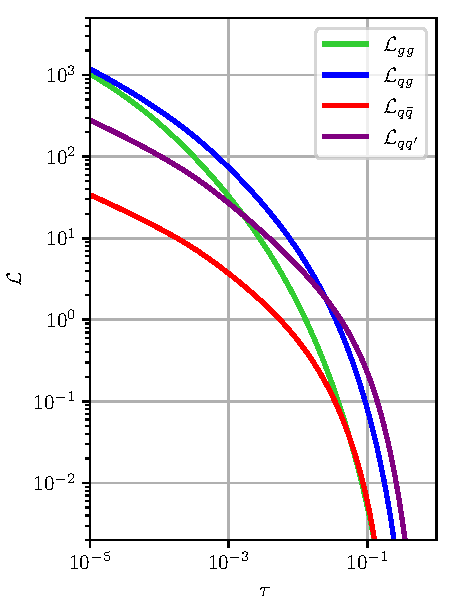
\includegraphics[width=\figurewidth]{Images/luminosity.pdf}
  \caption{Illustration of the partonic luminosity of parton $i$ and $j$. We choose exemplary parton combinations to represent gluon--gluon, gluon--valence-quark, gluon--sea-quark, valence-quark--sea-quark, valence-quark--valence-quark and sea-quark--sea-quark luminosities. For the luminosity of two different partons we include a factor $2$ to account for the different flavor permutations. The luminosity was calculated using the \texttt{LHAPDF6}~\cite{Buckley:2014ana} interface to the \texttt{NNPDF31\_nnlo\_as\_0118}~\cite{NNPDF:2017mvq} \acs{PDF} set at a scale of $\mu_F=m_H/2$ with a fixed collider energy of $\sqrt{S} = 13 \TeV$.}
\end{figure}

\section{The Leading-Order Cross Section}
Here I compute the leading-order cross section for Higgs Production in the gluon-gluon fusion channel.
\section{The Heavy-Top Limit}
Here I explain the heavy-top limit.
\section{Higher-Order Corrections}
Here I outline how to perform higher order corrections.
\section{Theory Status}
Here I describe what is already known about the gluon-gluon fusion channel. I explain the theory uncertainties.

